\documentclass[a4paper,10pt]{article}

\usepackage{tikz}
\usepackage{dblfnote}
\usepackage{lipsum}
\usepackage{tabularx}
\usepackage{graphicx}
\usepackage{multirow}

\usepackage{geometry}
\geometry{
    right=1cm,
    left=1cm,
    top=2cm,
    bottom=2cm
}

\usepackage{xepersian}
\settextfont{Vazirmatn-Regular.ttf}

\title{سوالات احتمالی میان‌ترم 2 درس الگوریتم‌های گراف (با پاسخ)}
\author{استاد مربوطه:\\سرکار خانم دکتر معصومه دامرودی \and به نوشته:\\محمد خورشیدی روزبهانی}
\date{}

\linespread{1.5}

\begin{document}

    \maketitle

    \paragraph{سوال:} تعاریف، قضایا، نتایج و کاربردهای درون اسلایدها را شرح دهید.

    \paragraph{پاسخ:} اﺑﺘﺪا ﺑﻪ ﺗﻌﺎرﯾﻒ ﻣﻮﺟﻮد در اﺳﻼﯾﺪﻫﺎ پرداخته ﺷﺪه و ﻣﻮارد ﺑﻪ تفکیک ﺗﻮﺿﯿﺢ داده میﺷﻮد.

    \begin{itemize}
        
        \item ارتباطی/پیوندی\footnote{\hspace{2pt}Connectivity}: در مفهوم گراف، ارتباطی/پیوندی یک مفهوم مهم است که به ارتباط و ارتباطات بین رئوس در یک گراف اشاره دارد.

        \item اجزای متصل\footnote{\hspace{2pt}Components Connected}: در مفهوم گراف، اجزای متصل به زیرمجموعه‌هایی از رئوس در یک گراف اشاره دارند که هر راس در هر اجزای متصل قابل دسترسی به همه‌ رئوس دیگر آن اجزا است، اما با رئوس اجزا دیگر قابل دسترسی نیستند. به عبارت دیگر، هر اجزای متصل به گونه‌ای با هم ارتباط دارند که می‌توان از هر راس در یک اجزای متصل به هر راس دیگر در همان اجزای متصل مسیری یافت.
        
        این مفهوم در تجزیه و تحلیل گراف‌ها و برخی مسائل کاربرد دارد، زیرا اجزای متصل می‌توانند به عنوان واحدهای اصلی در بررسی ساختار یک گراف مورد استفاده قرار گیرند.
        
        \item اتصال\footnote{\hspace{2pt}Connectedness}: مفهوم اتصال در یک گراف به وجود داشتن مسیر بین هر زوج رئوس در گراف اشاره دارد. به عبارت دیگر، یک گراف متصل است اگر بین هر دو راس دلخواهی در آن یک مسیر وجود داشته باشد.

        اگر یک گراف یک اجزای متصل داشته باشد، به عنوان یک واحد اتصالی در نظر گرفته می‌شود و به عنوان یک واحد کلی مورد بررسی قرار می‌گیرد. اگر یک گراف دو یا چند اجزای متصل داشته باشد، این گراف به عنوان یک گراف قطع شده محسوب می‌شود.

        اتصال در گراف‌ها به ما اطمینان می‌دهد که ارتباطات بین رئوس یا نقاط در گراف حفظ شده است و هیچ رئوسی از دسترسی به همسایگان خود محروم نیست. این مفهوم در بسیاری از برنامه‌ها و مسائلی مانند شبکه‌ها، مسائل جستجو، طراحی سیستم‌های ارتباطی، و غیره کاربرد دارد.

        \item بسیار متصل\footnote{\hspace{2pt}Connected Strongly}: یک گراف جهت‌دار\footnote{\hspace{2pt}Graph Directed} را می‌توان به عنوان «بسیار متصل» توصیف کرد اگر برای هر زوج رئوس مختلف $u$ و $v$ در گراف، یک مسیر از $u$ به $v$ و یک مسیر از $v$ به $u$ وجود داشته باشد. به طور دیگر، اگر بتوانیم از هر راس به هر راس دیگری در گراف دسترسی پیدا کنیم، آن گراف را بسیار متصل می‌نامیم.

        مفهوم بسیار متصل در گراف‌های جهت‌دار بسیار مهم است، به ویژه در مسائلی که ارتباطات جهت‌دار بین نقاط مهم هستند، مانند مسائل راه‌یابی و تحلیل شبکه‌های ارتباطی.

        \item اجزای بسیار متصل\footnote{\hspace{2pt}Component Connected Strongly (SCC)}: در واقع، این اصطلاح به یک زیرگراف جهت‌دار\footnote{\hspace{2pt}Subgraph Directed} از یک گراف اشاره دارد که تمام رئوس آن به یکدیگر متصل هستند و از هر راسی به هر راس دیگری در آن زیرگراف مسیر وجود دارد.

        \item کلاس اولیه\footnote{\hspace{2pt}Class Initial}: این مفهوم به راس یا رئوسی درون هر اجزای متصل اشاره دارد که هیچ یال ورودی ندارند. به عبارت دیگر، رئوسی که دریافت یال از رئوس دیگر را نمی‌کنند. این رئوس به عنوان نقاط شروع دیده می‌شوند که از آنجا پیمایش‌ها و ارتباطات درون کامپوننت شروع می‌شود.

        \item کلاس پایانی\footnote{\hspace{2pt}Class Final}: این مفهوم به راس یا رئوس درون هر اجزای متصل اشاره دارد که هیچ یال خروجی ندارند. به عبارت دیگر، رئوسی که هیچ یالی به رئوس دیگر بیرون از کامپوننت ارسال نمی‌کنند. این رئوس به عنوان نقاط پایانی مورد استفاده قرار می‌گیرند که پایان یافتن پیمایش‌ها و ارتباطات را نشان می‌دهند.
        
        \item کلاس میانی\footnote{\hspace{2pt}Class Intermediate}: راس یا رئوسی که هم یال ورودی و هم یال خروجی دارند و درون هر اجزای متصل وجود دارند، به عنوان رئوس میانی شناخته می‌شوند. این رئوس به عنوان مسیرهای انتقالی بین نقاط شروع و پایان درون یک کامپوننت عمل می‌کنند.

        \item برش راسی\footnote{\hspace{2pt}Vertex-Cut}: مفهوم برش راسی در گراف، یک مجموعه‌ای از رئوس یا گره‌ها است که با حذف آن‌ها، گراف به دو یا چندین قسمت جداگانه تقسیم می‌شود. به طور دقیق‌تر، اگر حذف یک مجموعه از رئوس باعث شود که گراف دیگر به‌طور متصل نباشد، آن مجموعه به عنوان یک برش رأسی شناخته می‌شود.
        
        \begin{center}
            
            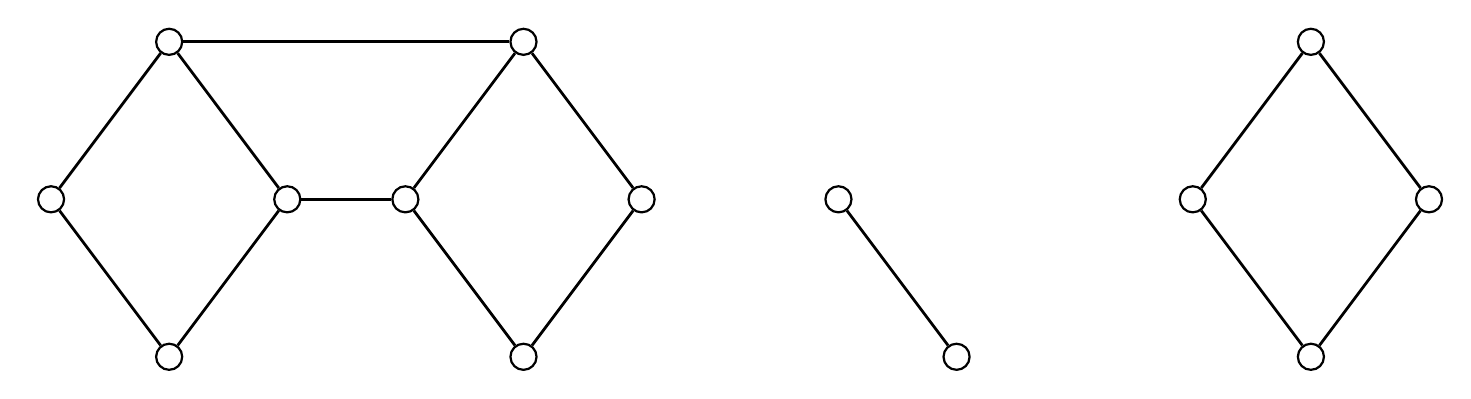
\begin{tikzpicture}

                \node[circle, draw, thick] (A) at (0,0) {};
                \node[circle, draw, thick] (B) at (1.5,2) {};
                \node[circle, draw, thick] (C) at (1.5,-2) {};
                \node[circle, draw, thick] (D) at (3,0) {};
                \node[circle, draw, thick] (E) at (4.5,0) {};
                \node[circle, draw, thick] (F) at (6,2) {};
                \node[circle, draw, thick] (G) at (6,-2) {};
                \node[circle, draw, thick] (H) at (7.5,0) {};
                
                \draw[line width=1pt] (A) -- (B);
                \draw[line width=1pt] (A) -- (C);
                \draw[line width=1pt] (B) -- (D);
                \draw[line width=1pt] (C) -- (D);
                \draw[line width=1pt] (E) -- (F);
                \draw[line width=1pt] (E) -- (G);
                \draw[line width=1pt] (F) -- (H);
                \draw[line width=1pt] (G) -- (H);
                \draw[line width=1pt] (B) -- (F);
                \draw[line width=1pt] (D) -- (E);

                \node[circle, draw, thick] (A) at (10,0) {};
                \node[circle, draw, thick] (C) at (11.5,-2) {};
                \node[circle, draw, thick] (E) at (14.5,0) {};
                \node[circle, draw, thick] (F) at (16,2) {};
                \node[circle, draw, thick] (G) at (16,-2) {};
                \node[circle, draw, thick] (H) at (17.5,0) {};

                \draw[line width=1pt] (A) -- (C);
                \draw[line width=1pt] (E) -- (F);
                \draw[line width=1pt] (E) -- (G);
                \draw[line width=1pt] (F) -- (H);
                \draw[line width=1pt] (G) -- (H);

            \end{tikzpicture}

        \end{center}

        \item برش یالی\footnote{\hspace{2pt}Edge-Cut}: در مفهوم گراف، یک برش یالی مجموعه‌ای از یال‌ها است که با حذف آن‌ها، گراف به دو یا چندین قسمت جداگانه تقسیم می‌شود. به طور دقیق‌تر، اگر حذف یک مجموعه از یال‌ها باعث شود که هیچ مسیری بین دو راس در دو قسمت متفاوت از گراف وجود نداشته باشد، آن مجموعه به عنوان یک برش یالی شناخته می‌شود.

        \begin{center}
            
            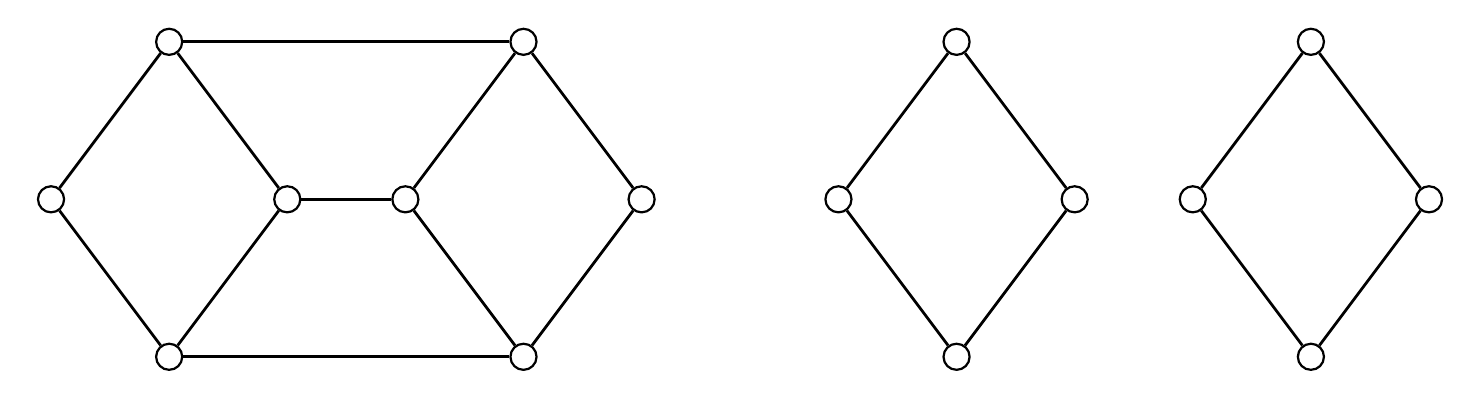
\begin{tikzpicture}

                \node[circle, draw, thick] (A) at (0,0) {};
                \node[circle, draw, thick] (B) at (1.5,2) {};
                \node[circle, draw, thick] (C) at (1.5,-2) {};
                \node[circle, draw, thick] (D) at (3,0) {};
                \node[circle, draw, thick] (E) at (4.5,0) {};
                \node[circle, draw, thick] (F) at (6,2) {};
                \node[circle, draw, thick] (G) at (6,-2) {};
                \node[circle, draw, thick] (H) at (7.5,0) {};
                
                \draw[line width=1pt] (A) -- (B);
                \draw[line width=1pt] (A) -- (C);
                \draw[line width=1pt] (B) -- (D);
                \draw[line width=1pt] (C) -- (D);
                \draw[line width=1pt] (E) -- (F);
                \draw[line width=1pt] (E) -- (G);
                \draw[line width=1pt] (F) -- (H);
                \draw[line width=1pt] (G) -- (H);
                \draw[line width=1pt] (B) -- (F);
                \draw[line width=1pt] (D) -- (E);
                \draw[line width=1pt] (C) -- (G);

                \node[circle, draw, thick] (A) at (10,0) {};
                \node[circle, draw, thick] (B) at (11.5,2) {};
                \node[circle, draw, thick] (C) at (11.5,-2) {};
                \node[circle, draw, thick] (D) at (13,0) {};
                \node[circle, draw, thick] (E) at (14.5,0) {};
                \node[circle, draw, thick] (F) at (16,2) {};
                \node[circle, draw, thick] (G) at (16,-2) {};
                \node[circle, draw, thick] (H) at (17.5,0) {};
                
                \draw[line width=1pt] (A) -- (B);
                \draw[line width=1pt] (A) -- (C);
                \draw[line width=1pt] (B) -- (D);
                \draw[line width=1pt] (C) -- (D);
                \draw[line width=1pt] (E) -- (F);
                \draw[line width=1pt] (E) -- (G);
                \draw[line width=1pt] (F) -- (H);
                \draw[line width=1pt] (G) -- (H);

            \end{tikzpicture}

        \end{center}

        \item مجموعه برش\footnote{\hspace{2pt}Cut-Set}: یک مجموعه برش، یک مجموعه برش حداقلی\footnote{\hspace{2pt}Cut-Set Minimal} نیز می‌باشد؛ یعنی حذف این مجموعه از یال‌ها باعث قطع شدن گراف و جدا شدن آن به دو یا چندین اجزای متصل می‌شود.
        
        یک مجموعه برش در گراف $G$ مجموعه‌ای از یال‌ها $F$ است که با حذف آن‌ها گراف قطع می‌شود، به شرطی که حذف هیچ زیرمجموعه مناسب\footnote{\hspace{2pt}Subset Proper} از $F$ نتواند گراف را قطع کند. این مجموعه برش حداقلی یا برش ساده\footnote{\hspace{2pt}Cut-Set Simple} نیز نامیده می‌شود. همچنین به عنوان برش مناسب یا چرخه مشترک\footnote{\hspace{2pt}Cocycle} نیز شناخته می‌شود.

        \item گراف جدایی‌پذیر\footnote{\hspace{2pt}Graph Separable}: گراف جدایی‌پذیر، به گرافی اشاره دارد که با حذف یک یا چند راس یا یال خاص، به دو یا چندین بخش مجزا تقسیم می‌شود. این گراف‌ها معمولاً دارای رئوسی هستند که به عنوان نقاط بحرانی یا برش راس عمل می‌کنند و با حذف آن‌ها، ساختار گراف به طور قابل توجهی تغییر می‌کند.

        \begin{center}
            
            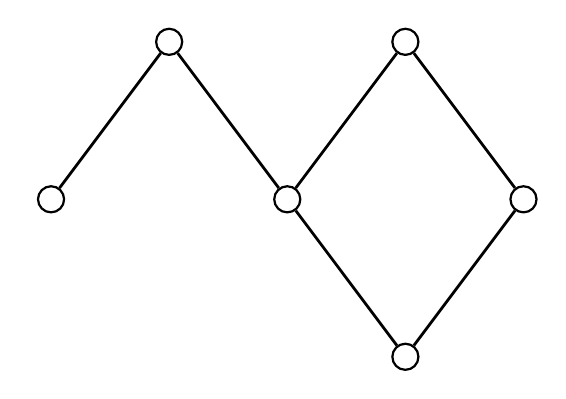
\begin{tikzpicture}
                
                \node[circle, draw, thick] (A) at (0,0) {};
                \node[circle, draw, thick] (B) at (1.5,2) {};
                \node[circle, draw, thick] (C) at (3,0) {};
                \node[circle, draw, thick] (D) at (4.5,2) {};
                \node[circle, draw, thick] (E) at (4.5,-2) {};
                \node[circle, draw, thick] (F) at (6,0) {};
                
                \draw[line width=1pt] (A) -- (B);
                \draw[line width=1pt] (B) -- (C);
                \draw[line width=1pt] (D) -- (C);
                \draw[line width=1pt] (E) -- (C);
                \draw[line width=1pt] (D) -- (F);
                \draw[line width=1pt] (E) -- (F);

            \end{tikzpicture}

        \end{center}

        \item گراف جدایی‌ناپذیر\footnote{\hspace{2pt}Graph Non-Separable}: گراف جدایی‌ناپذیر به گرافی گفته می‌شود که نمی‌توان آن را با حذف یک راس یا یال به دو یا چندین بخش مجزا تقسیم کرد. به عبارت دیگر، حذف هیچ راسی یا یالی باعث نمی‌شود که گراف قطع شود. این گراف‌ها ساختاری قوی و متصل دارند و نقاط بحرانی یا برش راس که باعث جداسازی گراف شوند، ندارند.

        \begin{center}
            
            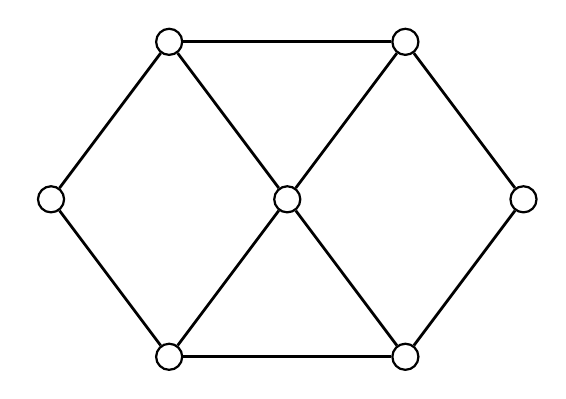
\begin{tikzpicture}
                
                \node[circle, draw, thick] (A) at (0,0) {};
                \node[circle, draw, thick] (B) at (1.5,2) {};
                \node[circle, draw, thick] (C) at (1.5,-2) {};
                \node[circle, draw, thick] (D) at (3,0) {};
                \node[circle, draw, thick] (E) at (4.5,2) {};
                \node[circle, draw, thick] (F) at (4.5,-2) {};
                \node[circle, draw, thick] (G) at (6,0) {};
                
                \draw[line width=1pt] (A) -- (B);
                \draw[line width=1pt] (A) -- (C);
                \draw[line width=1pt] (B) -- (D);
                \draw[line width=1pt] (C) -- (D);
                \draw[line width=1pt] (E) -- (D);
                \draw[line width=1pt] (F) -- (D);
                \draw[line width=1pt] (E) -- (G);
                \draw[line width=1pt] (F) -- (G);
                \draw[line width=1pt] (B) -- (E);
                \draw[line width=1pt] (C) -- (F);

            \end{tikzpicture}

        \end{center}

        \item بلوک\footnote{\hspace{2pt}Block}: بلوک یک زیرگراف جدایی‌ناپذیر از یک گراف جدایی‌پذیر $G$ است. به عبارت دیگر، بلوک یک زیرگراف متصل است که با حذف هیچ یک از رئوس آن (همراه با یال‌های متصل به آن راس) به بخش‌های مجزا تقسیم نمی‌شود.

        \begin{center}
            
            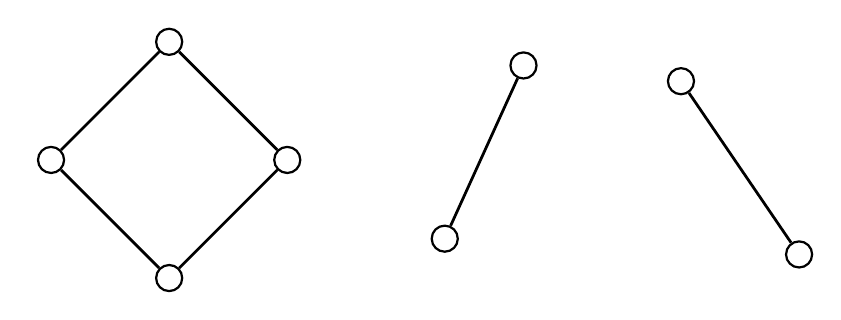
\begin{tikzpicture}
                
                \node[circle, draw, thick] (A) at (0,0) {};
                \node[circle, draw, thick] (B) at (1.5,1.5) {};
                \node[circle, draw, thick] (C) at (1.5,-1.5) {};
                \node[circle, draw, thick] (D) at (3,0) {};

                \draw[line width=1pt] (A) -- (B);
                \draw[line width=1pt] (A) -- (C);
                \draw[line width=1pt] (B) -- (D);
                \draw[line width=1pt] (C) -- (D);
                
                \node[circle, draw, thick] (A) at (5,-1) {};
                \node[circle, draw, thick] (B) at (6,1.2) {};

                \draw[line width=1pt] (A) -- (B);

                \node[circle, draw, thick] (A) at (9.5,-1.2) {};
                \node[circle, draw, thick] (B) at (8,1) {};

                \draw[line width=1pt] (A) -- (B);                

            \end{tikzpicture}

        \end{center}

        \item اتصال یالی\footnote{\hspace{2pt}Connectivity Edge}: مفهوم اتصال یالی در گراف به حداقل تعداد یال‌هایی که باید از گراف حذف شوند تا گراف به دو یا چندین اجزای متصل جداگانه تقسیم شود، اشاره دارد. به عبارت دیگر، اتصال یالی گراف نشان‌دهنده‌ میزان پایداری گراف در برابر حذف یال‌ها است.

        به عبارت دیگر، اتصال یالی حداقل تعداد یال‌هایی است که باید حذف شوند تا گراف به یک گراف قطع تبدیل شود. این مقدار به عنوان $\lambda (G)$ نشان داده می‌شود.

        \item اتصال راسی\footnote{\hspace{2pt}Connectivity Vertex}: مفهوم اتصال راسی در گراف به حداقل تعداد رئوسی که باید از گراف حذف شوند تا گراف به دو یا چندین بخش مجزا تقسیم شود، اشاره دارد. این مفهوم میزان پایداری گراف را در برابر حذف رئوس نشان می‌دهد.
        
        به عبارت دیگر، اتصال راسی حداقل تعداد رئوسی است که باید حذف شوند تا گراف به یک گراف قطع تبدیل شود. این مقدار به عنوان $\kappa (G)$ نشان داده می‌شود.

        \item جستجوی عمق اول\footnote{\hspace{2pt}Search First Depth (DFS)}: جستجوی عمق‌ اول یک الگوریتم پیمایش یا جستجو در ساختارهای داده‌ای مانند گراف‌ها و درخت‌ها است. این الگوریتم به طور عمیق در ساختار حرکت می‌کند و تا زمانی که به یک رأس یا گره بدون فرزند نرسد، به پیشروی ادامه می‌دهد. سپس به عقب برگشته و به دنبال مسیرهای دیگر می‌گردد.
        
        به عنوان مثال می‌توان گراف زیر را در نظر گرفت و با توجه به گراف زیر الگوریتم جستجوی عمق اول را برای آن به صورت زیر نوشت.

        \begin{table}
            
            \centering
            \begin{tabular}{ c c }
                
                \begin{tabular}{ r c }

                    لیست & دیده شده \\

                    \hline
                
                    \{\textcolor{blue}{2}\} & 2 \\
                    \{2, \textcolor{blue}{1}\} & 1 \\
                    \{2, 1, \textcolor{blue}{4}\} & 4 \\
                    \{2, 1, 4, \textcolor{blue}{3}\} & 3 \\
                    \{2, 1, 4, 3, \textcolor{blue}{7}\} & 7 \\
                    \{2, 1, 4, \textcolor{blue}{3}\} &  \\
                    \{2, 1, 4, 3, \textcolor{blue}{8}\} & 8 \\
                    \{2, 1, 4, \textcolor{blue}{3}\} &  \\
                    \{2, 1, \textcolor{blue}{4}\} &  \\
                    \{2, 1, 4, \textcolor{blue}{6}\} & 6 \\
                    \{2, 1, 4, 6, \textcolor{blue}{5}\} & 5 \\
                    \{2, 1, 4, \textcolor{blue}{6}\} &  \\
                    \{2, 1, \textcolor{blue}{4}\} &  \\
                    \{2, \textcolor{blue}{1}\} &  \\
                    \{\textcolor{blue}{2}\} &  \\
                    \{\} &  \\
                
                \end{tabular}

                &

                \begin{tabular}{ c c }
                    
                    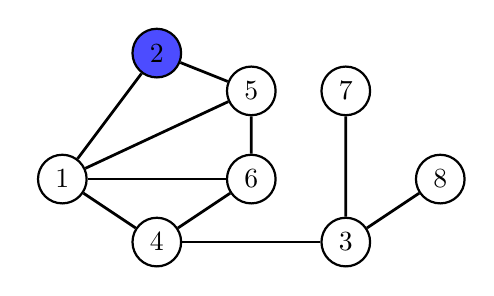
\begin{tikzpicture}[scale=0.8]
                
                        \node[circle, draw, thick] (1) at (0,0) {1};
                        \node[circle, fill=blue!70, draw, thick] (2) at (1.5,2) {2};
                        \node[circle, draw, thick] (3) at (4.5,-1) {3};
                        \node[circle, draw, thick] (4) at (1.5,-1) {4};
                        \node[circle, draw, thick] (5) at (3,1.4) {5};
                        \node[circle, draw, thick] (6) at (3,0) {6};
                        \node[circle, draw, thick] (7) at (4.5,1.4) {7};
                        \node[circle, draw, thick] (8) at (6,0) {8};
        
                        \draw[line width=1] (1) -- (2);
                        \draw[line width=1] (1) -- (5);
                        \draw[line width=1] (1) -- (6);
                        \draw[line width=1] (1) -- (4);
                        \draw[line width=1] (5) -- (2);
                        \draw[line width=1] (5) -- (6);
                        \draw[line width=1] (4) -- (6);
                        \draw[line width=1] (4) -- (3);
                        \draw[line width=1] (8) -- (3);
                        \draw[line width=1] (7) -- (3);
        
                    \end{tikzpicture}

                    &

                    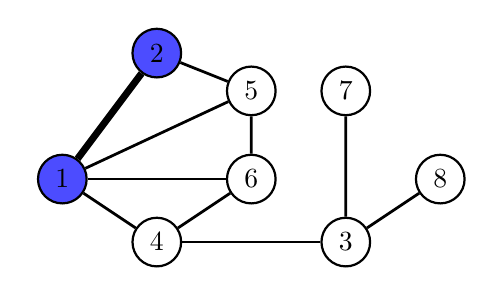
\begin{tikzpicture}[scale=0.8]
                
                        \node[circle, fill=blue!70, draw, thick] (1) at (0,0) {1};
                        \node[circle, fill=blue!70, draw, thick] (2) at (1.5,2) {2};
                        \node[circle, draw, thick] (3) at (4.5,-1) {3};
                        \node[circle, draw, thick] (4) at (1.5,-1) {4};
                        \node[circle, draw, thick] (5) at (3,1.4) {5};
                        \node[circle, draw, thick] (6) at (3,0) {6};
                        \node[circle, draw, thick] (7) at (4.5,1.4) {7};
                        \node[circle, draw, thick] (8) at (6,0) {8};
        
                        \draw[line width=2.5] (1) -- (2);
                        \draw[line width=1] (1) -- (5);
                        \draw[line width=1] (1) -- (6);
                        \draw[line width=1] (1) -- (4);
                        \draw[line width=1] (5) -- (2);
                        \draw[line width=1] (5) -- (6);
                        \draw[line width=1] (4) -- (6);
                        \draw[line width=1] (4) -- (3);
                        \draw[line width=1] (8) -- (3);
                        \draw[line width=1] (7) -- (3);
        
                    \end{tikzpicture} \\

                    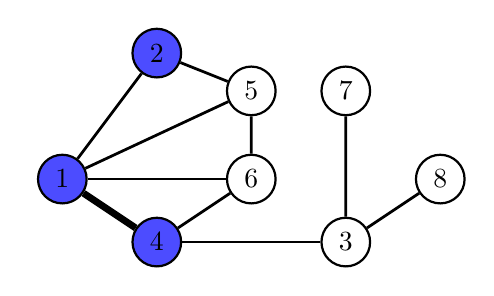
\begin{tikzpicture}[scale=0.8]
                
                        \node[circle, fill=blue!70, draw, thick] (1) at (0,0) {1};
                        \node[circle, fill=blue!70, draw, thick] (2) at (1.5,2) {2};
                        \node[circle, draw, thick] (3) at (4.5,-1) {3};
                        \node[circle, fill=blue!70, draw, thick] (4) at (1.5,-1) {4};
                        \node[circle, draw, thick] (5) at (3,1.4) {5};
                        \node[circle, draw, thick] (6) at (3,0) {6};
                        \node[circle, draw, thick] (7) at (4.5,1.4) {7};
                        \node[circle, draw, thick] (8) at (6,0) {8};
        
                        \draw[line width=1] (1) -- (2);
                        \draw[line width=1] (1) -- (5);
                        \draw[line width=1] (1) -- (6);
                        \draw[line width=2.5] (1) -- (4);
                        \draw[line width=1] (5) -- (2);
                        \draw[line width=1] (5) -- (6);
                        \draw[line width=1] (4) -- (6);
                        \draw[line width=1] (4) -- (3);
                        \draw[line width=1] (8) -- (3);
                        \draw[line width=1] (7) -- (3);
        
                    \end{tikzpicture}

                    &

                    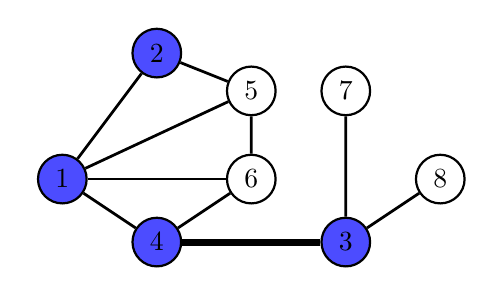
\begin{tikzpicture}[scale=0.8]
                
                        \node[circle, fill=blue!70, draw, thick] (1) at (0,0) {1};
                        \node[circle, fill=blue!70, draw, thick] (2) at (1.5,2) {2};
                        \node[circle, fill=blue!70, draw, thick] (3) at (4.5,-1) {3};
                        \node[circle, fill=blue!70, draw, thick] (4) at (1.5,-1) {4};
                        \node[circle, draw, thick] (5) at (3,1.4) {5};
                        \node[circle, draw, thick] (6) at (3,0) {6};
                        \node[circle, draw, thick] (7) at (4.5,1.4) {7};
                        \node[circle, draw, thick] (8) at (6,0) {8};
        
                        \draw[line width=1] (1) -- (2);
                        \draw[line width=1] (1) -- (5);
                        \draw[line width=1] (1) -- (6);
                        \draw[line width=1] (1) -- (4);
                        \draw[line width=1] (5) -- (2);
                        \draw[line width=1] (5) -- (6);
                        \draw[line width=1] (4) -- (6);
                        \draw[line width=2.5] (4) -- (3);
                        \draw[line width=1] (8) -- (3);
                        \draw[line width=1] (7) -- (3);
        
                    \end{tikzpicture} \\

                    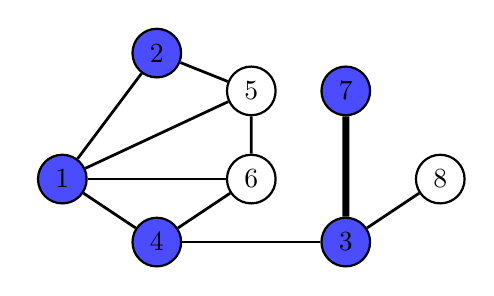
\begin{tikzpicture}[scale=0.8]
                
                        \node[circle, fill=blue!70, draw, thick] (1) at (0,0) {1};
                        \node[circle, fill=blue!70, draw, thick] (2) at (1.5,2) {2};
                        \node[circle, fill=blue!70, draw, thick] (3) at (4.5,-1) {3};
                        \node[circle, fill=blue!70, draw, thick] (4) at (1.5,-1) {4};
                        \node[circle, draw, thick] (5) at (3,1.4) {5};
                        \node[circle, draw, thick] (6) at (3,0) {6};
                        \node[circle, fill=blue!70, draw, thick] (7) at (4.5,1.4) {7};
                        \node[circle, draw, thick] (8) at (6,0) {8};
        
                        \draw[line width=1] (1) -- (2);
                        \draw[line width=1] (1) -- (5);
                        \draw[line width=1] (1) -- (6);
                        \draw[line width=1] (1) -- (4);
                        \draw[line width=1] (5) -- (2);
                        \draw[line width=1] (5) -- (6);
                        \draw[line width=1] (4) -- (6);
                        \draw[line width=1] (4) -- (3);
                        \draw[line width=1] (8) -- (3);
                        \draw[line width=2.5] (7) -- (3);
        
                    \end{tikzpicture}

                    &

                    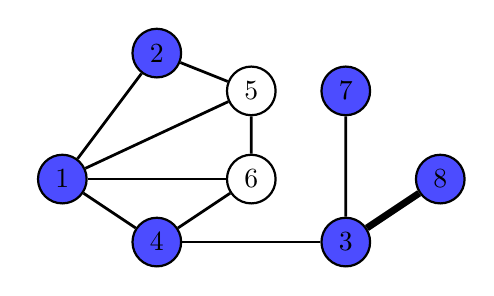
\begin{tikzpicture}[scale=0.8]
                
                        \node[circle, fill=blue!70, draw, thick] (1) at (0,0) {1};
                        \node[circle, fill=blue!70, draw, thick] (2) at (1.5,2) {2};
                        \node[circle, fill=blue!70, draw, thick] (3) at (4.5,-1) {3};
                        \node[circle, fill=blue!70, draw, thick] (4) at (1.5,-1) {4};
                        \node[circle, draw, thick] (5) at (3,1.4) {5};
                        \node[circle, draw, thick] (6) at (3,0) {6};
                        \node[circle, fill=blue!70, draw, thick] (7) at (4.5,1.4) {7};
                        \node[circle, fill=blue!70, draw, thick] (8) at (6,0) {8};
        
                        \draw[line width=1] (1) -- (2);
                        \draw[line width=1] (1) -- (5);
                        \draw[line width=1] (1) -- (6);
                        \draw[line width=1] (1) -- (4);
                        \draw[line width=1] (5) -- (2);
                        \draw[line width=1] (5) -- (6);
                        \draw[line width=1] (4) -- (6);
                        \draw[line width=1] (4) -- (3);
                        \draw[line width=2.5] (8) -- (3);
                        \draw[line width=1] (7) -- (3);
        
                    \end{tikzpicture} \\

                    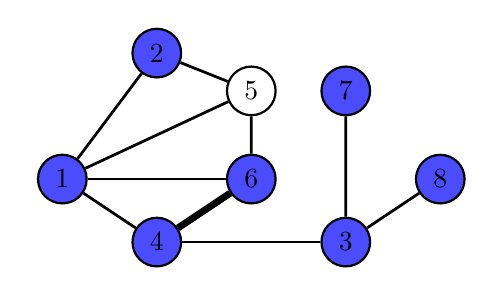
\begin{tikzpicture}[scale=0.8]
                
                        \node[circle, fill=blue!70, draw, thick] (1) at (0,0) {1};
                        \node[circle, fill=blue!70, draw, thick] (2) at (1.5,2) {2};
                        \node[circle, fill=blue!70, draw, thick] (3) at (4.5,-1) {3};
                        \node[circle, fill=blue!70, draw, thick] (4) at (1.5,-1) {4};
                        \node[circle, draw, thick] (5) at (3,1.4) {5};
                        \node[circle, fill=blue!70, draw, thick] (6) at (3,0) {6};
                        \node[circle, fill=blue!70, draw, thick] (7) at (4.5,1.4) {7};
                        \node[circle, fill=blue!70, draw, thick] (8) at (6,0) {8};
        
                        \draw[line width=1] (1) -- (2);
                        \draw[line width=1] (1) -- (5);
                        \draw[line width=1] (1) -- (6);
                        \draw[line width=1] (1) -- (4);
                        \draw[line width=1] (5) -- (2);
                        \draw[line width=1] (5) -- (6);
                        \draw[line width=2.5] (4) -- (6);
                        \draw[line width=1] (4) -- (3);
                        \draw[line width=1] (8) -- (3);
                        \draw[line width=1] (7) -- (3);
        
                    \end{tikzpicture}

                    &

                    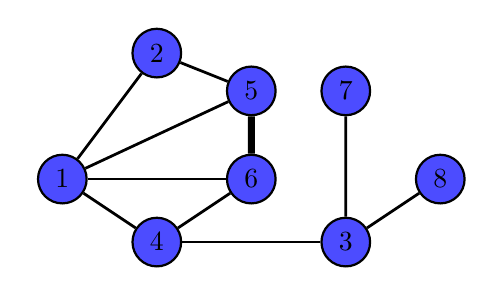
\begin{tikzpicture}[scale=0.8]
                
                        \node[circle, fill=blue!70, draw, thick] (1) at (0,0) {1};
                        \node[circle, fill=blue!70, draw, thick] (2) at (1.5,2) {2};
                        \node[circle, fill=blue!70, draw, thick] (3) at (4.5,-1) {3};
                        \node[circle, fill=blue!70, draw, thick] (4) at (1.5,-1) {4};
                        \node[circle, fill=blue!70, draw, thick] (5) at (3,1.4) {5};
                        \node[circle, fill=blue!70, draw, thick] (6) at (3,0) {6};
                        \node[circle, fill=blue!70, draw, thick] (7) at (4.5,1.4) {7};
                        \node[circle, fill=blue!70, draw, thick] (8) at (6,0) {8};
        
                        \draw[line width=1] (1) -- (2);
                        \draw[line width=1] (1) -- (5);
                        \draw[line width=1] (1) -- (6);
                        \draw[line width=1] (1) -- (4);
                        \draw[line width=1] (5) -- (2);
                        \draw[line width=2.5] (5) -- (6);
                        \draw[line width=1] (4) -- (6);
                        \draw[line width=1] (4) -- (3);
                        \draw[line width=1] (8) -- (3);
                        \draw[line width=1] (7) -- (3);
        
                    \end{tikzpicture} \\
                    
                \end{tabular} \\

            \end{tabular}
            \caption{جستجوی عمق اول}

        \end{table}

        \item جستجوی عرض اول\footnote{\hspace{2pt}Search First Breadth (BFS)}: جستجوی عرض‌ اول یک الگوریتم پیمایش یا جستجو در ساختارهای داده‌ای مانند گراف‌ها و درخت‌ها است. این الگوریتم به جای پیمایش عمقی، به پیمایش سطحی می‌پردازد، به این معنا که ابتدا همه رئوس هم‌سطح را پیمایش می‌کند و سپس به سطح بعدی می‌رود.

        \begin{table}
            
            \centering
            \begin{tabular}{ c c }
                
                \begin{tabular}{ r c }

                    لیست & دیده شده \\

                    \hline
                
                    \{\textcolor{blue}{2}\} & 2 \\
                    \{\textcolor{blue}{2}, 1\} & 1 \\
                    \{\textcolor{blue}{2}, 1, 5\} & 5 \\
                    \{\textcolor{blue}{1}, 5\} &  \\
                    \{\textcolor{blue}{1}, 5, 4\} & 4 \\
                    \{\textcolor{blue}{1}, 5, 4, 6\} & 6 \\
                    \{\textcolor{blue}{5}, 4, 6\} &  \\
                    \{\textcolor{blue}{4}, 6\} &  \\
                    \{\textcolor{blue}{4}, 6, 3\} & 3 \\
                    \{\textcolor{blue}{6}, 3\} &  \\
                    \{\textcolor{blue}{3}\} &  \\
                    \{\textcolor{blue}{3}, 7\} & 7 \\
                    \{\textcolor{blue}{3}, 7, 8\} & 8 \\
                    \{\textcolor{blue}{7}, 8\} &  \\
                    \{\textcolor{blue}{8}\} &  \\
                    \{\} &  \\
                
                \end{tabular}

                &

                \begin{tabular}{ c c }
                    
                    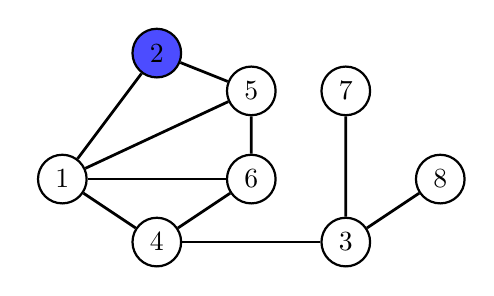
\begin{tikzpicture}[scale=0.8]
                
                        \node[circle, draw, thick] (1) at (0,0) {1};
                        \node[circle, fill=blue!70, draw, thick] (2) at (1.5,2) {2};
                        \node[circle, draw, thick] (3) at (4.5,-1) {3};
                        \node[circle, draw, thick] (4) at (1.5,-1) {4};
                        \node[circle, draw, thick] (5) at (3,1.4) {5};
                        \node[circle, draw, thick] (6) at (3,0) {6};
                        \node[circle, draw, thick] (7) at (4.5,1.4) {7};
                        \node[circle, draw, thick] (8) at (6,0) {8};
        
                        \draw[line width=1] (1) -- (2);
                        \draw[line width=1] (1) -- (5);
                        \draw[line width=1] (1) -- (6);
                        \draw[line width=1] (1) -- (4);
                        \draw[line width=1] (5) -- (2);
                        \draw[line width=1] (5) -- (6);
                        \draw[line width=1] (4) -- (6);
                        \draw[line width=1] (4) -- (3);
                        \draw[line width=1] (8) -- (3);
                        \draw[line width=1] (7) -- (3);
        
                    \end{tikzpicture}

                    &

                    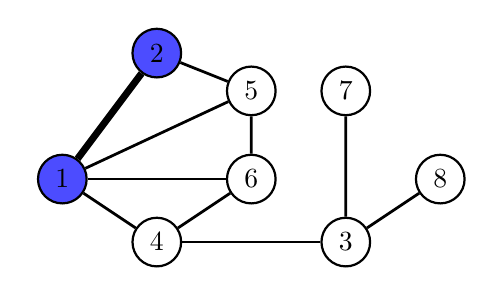
\begin{tikzpicture}[scale=0.8]
                
                        \node[circle, fill=blue!70, draw, thick] (1) at (0,0) {1};
                        \node[circle, fill=blue!70, draw, thick] (2) at (1.5,2) {2};
                        \node[circle, draw, thick] (3) at (4.5,-1) {3};
                        \node[circle, draw, thick] (4) at (1.5,-1) {4};
                        \node[circle, draw, thick] (5) at (3,1.4) {5};
                        \node[circle, draw, thick] (6) at (3,0) {6};
                        \node[circle, draw, thick] (7) at (4.5,1.4) {7};
                        \node[circle, draw, thick] (8) at (6,0) {8};
        
                        \draw[line width=2.5] (1) -- (2);
                        \draw[line width=1] (1) -- (5);
                        \draw[line width=1] (1) -- (6);
                        \draw[line width=1] (1) -- (4);
                        \draw[line width=1] (5) -- (2);
                        \draw[line width=1] (5) -- (6);
                        \draw[line width=1] (4) -- (6);
                        \draw[line width=1] (4) -- (3);
                        \draw[line width=1] (8) -- (3);
                        \draw[line width=1] (7) -- (3);
        
                    \end{tikzpicture} \\

                    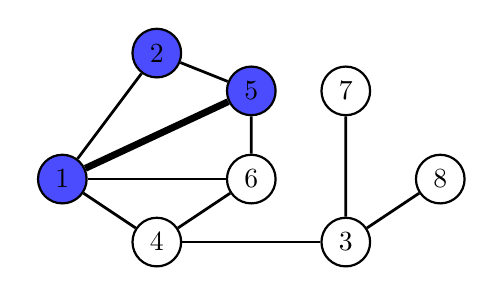
\begin{tikzpicture}[scale=0.8]
                
                        \node[circle, fill=blue!70, draw, thick] (1) at (0,0) {1};
                        \node[circle, fill=blue!70, draw, thick] (2) at (1.5,2) {2};
                        \node[circle, draw, thick] (3) at (4.5,-1) {3};
                        \node[circle, draw, thick] (4) at (1.5,-1) {4};
                        \node[circle, fill=blue!70, draw, thick] (5) at (3,1.4) {5};
                        \node[circle, draw, thick] (6) at (3,0) {6};
                        \node[circle, draw, thick] (7) at (4.5,1.4) {7};
                        \node[circle, draw, thick] (8) at (6,0) {8};
        
                        \draw[line width=1] (1) -- (2);
                        \draw[line width=2.5] (1) -- (5);
                        \draw[line width=1] (1) -- (6);
                        \draw[line width=1] (1) -- (4);
                        \draw[line width=1] (5) -- (2);
                        \draw[line width=1] (5) -- (6);
                        \draw[line width=1] (4) -- (6);
                        \draw[line width=1] (4) -- (3);
                        \draw[line width=1] (8) -- (3);
                        \draw[line width=1] (7) -- (3);
        
                    \end{tikzpicture}

                    &

                    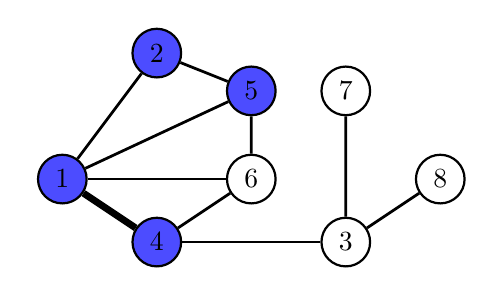
\begin{tikzpicture}[scale=0.8]
                
                        \node[circle, fill=blue!70, draw, thick] (1) at (0,0) {1};
                        \node[circle, fill=blue!70, draw, thick] (2) at (1.5,2) {2};
                        \node[circle, draw, thick] (3) at (4.5,-1) {3};
                        \node[circle, fill=blue!70, draw, thick] (4) at (1.5,-1) {4};
                        \node[circle, fill=blue!70, draw, thick] (5) at (3,1.4) {5};
                        \node[circle, draw, thick] (6) at (3,0) {6};
                        \node[circle, draw, thick] (7) at (4.5,1.4) {7};
                        \node[circle, draw, thick] (8) at (6,0) {8};
        
                        \draw[line width=1] (1) -- (2);
                        \draw[line width=1] (1) -- (5);
                        \draw[line width=1] (1) -- (6);
                        \draw[line width=2.5] (1) -- (4);
                        \draw[line width=1] (5) -- (2);
                        \draw[line width=1] (5) -- (6);
                        \draw[line width=1] (4) -- (6);
                        \draw[line width=1] (4) -- (3);
                        \draw[line width=1] (8) -- (3);
                        \draw[line width=1] (7) -- (3);
        
                    \end{tikzpicture} \\

                    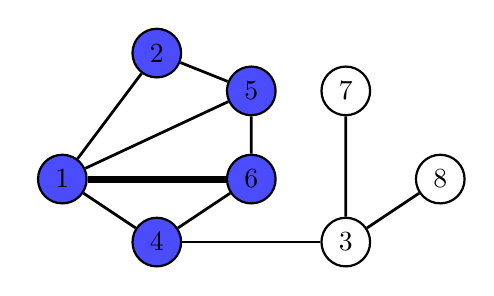
\begin{tikzpicture}[scale=0.8]
                
                        \node[circle, fill=blue!70, draw, thick] (1) at (0,0) {1};
                        \node[circle, fill=blue!70, draw, thick] (2) at (1.5,2) {2};
                        \node[circle, draw, thick] (3) at (4.5,-1) {3};
                        \node[circle, fill=blue!70, draw, thick] (4) at (1.5,-1) {4};
                        \node[circle, fill=blue!70, draw, thick] (5) at (3,1.4) {5};
                        \node[circle, fill=blue!70, draw, thick] (6) at (3,0) {6};
                        \node[circle, draw, thick] (7) at (4.5,1.4) {7};
                        \node[circle, draw, thick] (8) at (6,0) {8};
        
                        \draw[line width=1] (1) -- (2);
                        \draw[line width=1] (1) -- (5);
                        \draw[line width=2.5] (1) -- (6);
                        \draw[line width=1] (1) -- (4);
                        \draw[line width=1] (5) -- (2);
                        \draw[line width=1] (5) -- (6);
                        \draw[line width=1] (4) -- (6);
                        \draw[line width=1] (4) -- (3);
                        \draw[line width=1] (8) -- (3);
                        \draw[line width=1] (7) -- (3);
        
                    \end{tikzpicture}

                    &

                    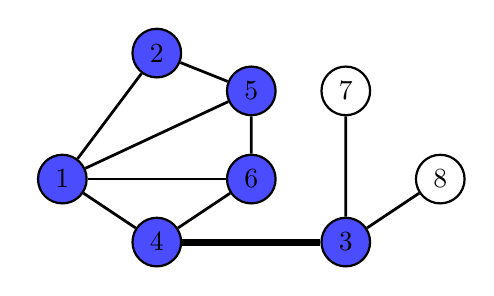
\begin{tikzpicture}[scale=0.8]
                
                        \node[circle, fill=blue!70, draw, thick] (1) at (0,0) {1};
                        \node[circle, fill=blue!70, draw, thick] (2) at (1.5,2) {2};
                        \node[circle, fill=blue!70, draw, thick] (3) at (4.5,-1) {3};
                        \node[circle, fill=blue!70, draw, thick] (4) at (1.5,-1) {4};
                        \node[circle, fill=blue!70, draw, thick] (5) at (3,1.4) {5};
                        \node[circle, fill=blue!70, draw, thick] (6) at (3,0) {6};
                        \node[circle, draw, thick] (7) at (4.5,1.4) {7};
                        \node[circle, draw, thick] (8) at (6,0) {8};
        
                        \draw[line width=1] (1) -- (2);
                        \draw[line width=1] (1) -- (5);
                        \draw[line width=1] (1) -- (6);
                        \draw[line width=1] (1) -- (4);
                        \draw[line width=1] (5) -- (2);
                        \draw[line width=1] (5) -- (6);
                        \draw[line width=1] (4) -- (6);
                        \draw[line width=2.5] (4) -- (3);
                        \draw[line width=1] (8) -- (3);
                        \draw[line width=1] (7) -- (3);
        
                    \end{tikzpicture} \\

                    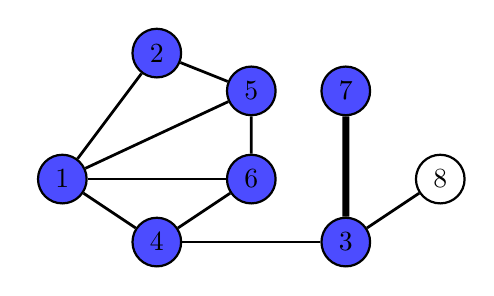
\begin{tikzpicture}[scale=0.8]
                
                        \node[circle, fill=blue!70, draw, thick] (1) at (0,0) {1};
                        \node[circle, fill=blue!70, draw, thick] (2) at (1.5,2) {2};
                        \node[circle, fill=blue!70, draw, thick] (3) at (4.5,-1) {3};
                        \node[circle, fill=blue!70, draw, thick] (4) at (1.5,-1) {4};
                        \node[circle, fill=blue!70, draw, thick] (5) at (3,1.4) {5};
                        \node[circle, fill=blue!70, draw, thick] (6) at (3,0) {6};
                        \node[circle, fill=blue!70, draw, thick] (7) at (4.5,1.4) {7};
                        \node[circle, draw, thick] (8) at (6,0) {8};
        
                        \draw[line width=1] (1) -- (2);
                        \draw[line width=1] (1) -- (5);
                        \draw[line width=1] (1) -- (6);
                        \draw[line width=1] (1) -- (4);
                        \draw[line width=1] (5) -- (2);
                        \draw[line width=1] (5) -- (6);
                        \draw[line width=1] (4) -- (6);
                        \draw[line width=1] (4) -- (3);
                        \draw[line width=1] (8) -- (3);
                        \draw[line width=2.5] (7) -- (3);
        
                    \end{tikzpicture}

                    &

                    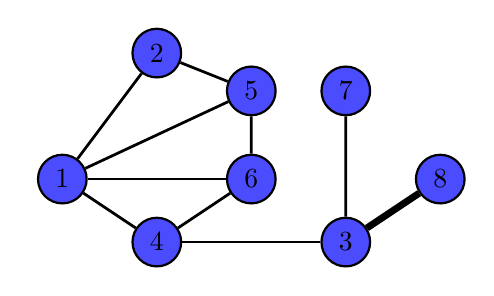
\begin{tikzpicture}[scale=0.8]
                
                        \node[circle, fill=blue!70, draw, thick] (1) at (0,0) {1};
                        \node[circle, fill=blue!70, draw, thick] (2) at (1.5,2) {2};
                        \node[circle, fill=blue!70, draw, thick] (3) at (4.5,-1) {3};
                        \node[circle, fill=blue!70, draw, thick] (4) at (1.5,-1) {4};
                        \node[circle, fill=blue!70, draw, thick] (5) at (3,1.4) {5};
                        \node[circle, fill=blue!70, draw, thick] (6) at (3,0) {6};
                        \node[circle, fill=blue!70, draw, thick] (7) at (4.5,1.4) {7};
                        \node[circle, fill=blue!70, draw, thick] (8) at (6,0) {8};
        
                        \draw[line width=1] (1) -- (2);
                        \draw[line width=1] (1) -- (5);
                        \draw[line width=1] (1) -- (6);
                        \draw[line width=1] (1) -- (4);
                        \draw[line width=1] (5) -- (2);
                        \draw[line width=1] (5) -- (6);
                        \draw[line width=1] (4) -- (6);
                        \draw[line width=1] (4) -- (3);
                        \draw[line width=2.5] (8) -- (3);
                        \draw[line width=1] (7) -- (3);
        
                    \end{tikzpicture} \\

                \end{tabular} \\

            \end{tabular}
            \caption{جستجوی عرض اول}

        \end{table}

    \end{itemize}

    

\end{document}